\documentclass[conference]{IEEEtran}
\usepackage{cite}
\usepackage{graphicx}
\usepackage{placeins}
\usepackage{caption}
\usepackage{subfigure}
\usepackage{enumerate}
\usepackage{afterpage}
\usepackage[font={small}]{caption}
\AtBeginDocument{\renewcommand{\abstractname}{Resumo}}
\begin{document}
\title{Projeto 1 de Introdu\c{c}\~ao ao Processamento de Imagens \\ Quinta Parte}
\author{\IEEEauthorblockN{Gabriel Martins de Miranda}
\IEEEauthorblockA{130111350\\
Universidade de Bras\'ilia\\
Email:gabrielmirandat@hotmail.com}
}
\maketitle
\begin{abstract}
O presente experimento realiza a filtragem da imagem $characters\_test\_pattern$ com filtros passa altas e passa baixas. Foram implementados dois modelos de filtros : $ideal $ e $Butterworth$.  
\end{abstract}

\section{ Introdu\c{c}\~ao} 
\label{sec:meth} 
Algumas considera\c{c}\~oes sobre a $Transformada$ $de$ $Fourier$. Atrav\'es da Transformada, sinais no dom\'inio do tempo s\~ao representados no dom\'inio da frequ\^encia. Atrav\'es disto obtemos o $espectro$ $de$ $frequencia$, e este subsivide$-$se em $espectro$ $de$ $amplitude$ e em  $espectro$ $de$ $fase$. As opera\c{c}\~oes de Fourier fazem aproxima\c{c}\~oes de fun\c{c}\~oes em intervalos definidos por um somat\'orio de senos e cossenos, em que o primeiro termo em geral representa a componente $dc$ do sinal e os outros as componentes $ac$.  \'E usada a $Serie$ $de$ $Fourier$ para representar sinais $periodicos$ e a $Transformada$ $de$ $Fourier$ propriamente dita para sinais $aperiodicos$. Ambas subdividem$-$se em :

\begin{itemize}
	\item S\'erie de Fourier:
	\begin{enumerate}[(a)]
		\item Sinal de tempo cont\'inuo
		\\
		$FS$ - S\'erie de Fourier
		\item Sinal de tempo discreto
		\\
		$DTFS$ - S\'erie de Fourier de tempo discreto
	\end{enumerate}
	\item Transformada de Fourier:
	\begin{enumerate}[(a)]
		\item Sinal de tempo cont\'inuo
		\\
		$FT$ - Transformada de Fourier 
		\item Sinal de tempo discreto
		\\
		$DTFT$ - Transformada de Fourier de tempo discreto
	\end{enumerate}
\end{itemize}
\vspace{2\baselineskip}\vspace{-\parskip}
Como o computador digital trabalha apenas com valores discretos, usaremos o modelo da $DTFS$, tamb\'em chamada de $Transformada $ $Discreta $ $de $ $Fourier$ = $DFT$ para trabalhar com imagens digitais. Para o proposto experimento, mais especificamente, ser\'a usada a  $Transformada $ $Rapida $ $de $ $Fourier$ = $FFT$, um algoritmo de baixa complexidade computacional  relativa para se calcular a Transformada Discreta de Fourier, que se baseia no m\'etodo chamado $metodo $ $dos $ $dobramentos $ $sucessivos$.
 
\section{Metodologia} 
\label{sec:meth} 
Para resolu\c{c}\~ao do problema seguiu$-$se os seguintes passos:

\begin{itemize}
	\item A imagem $f$ =  $characters\_test\_pattern$ foi lida pelo Matlab.
	\item Realizou$-$se o preenchimento na $f$ = $fpa$. De forma que $fpa$ passou a ter o dobro do tamanho(do n\'umero de linhas e colunas) de $f $ e $f$ a ocupar o centro da $fpa$. O procedimento foi realizado pela fun\c{c}\~ao $preenchimento.m$.
	\item Foi calculada a $DFT$ de $fpa$ = $Fpa$ atrav\'es da fun\c{c}\~ao $fft2$ do Matlab.
	\item $Fpa $ foi deslocada para concentrar as baixas frequ\^encias (maior parte do espectro) da imagem no centro = $Fpad$ atrav\'es da fun\c{c}\~ao $fftshift$ do Matlab. 
	\item Para i=1 at\'e 4, sendo (1 = ideal passa baixas, 2 = ideal passa altas, 3 = butterworth passa baixas, 4 = butterworth passa altas):
		\begin{enumerate}[(a)]
		\item $Fpad$ \'e mandada para a fun\c{c}\~ao cujo nome \'e o nome do filtro e esta retorna o produto de $Fpad$ com o filtro correspondente = $Gpad\_i$. As fun\c{c}\~oes s\~ao( $ideal\_passa\_baixas.m$,$ideal\_passa\_altas.m$,\\$Butterworth\_passa\_baixas.m$,$Butterworth\_passa\_altas.m$).
		\item O deslocamento foi desfeito em  $Gpad\_i$ = $Gpa\_i$ atrav\'es da fun\c{c}\~ao $ifftshift$ do Matlab.
		\item Aplicou$-$se $DFT$ inversa em $Gpa\_i$ = $gpa\_i$ atrav\'es da fun\c{c}\~ao $ifft2$ do Matlab.
		\item O preenchimento foi desfeito em  $gpa\_i$ = $g\_i$.O procedimento foi realizado pela fun\c{c}\~ao $despreenchimento.m$.
		\item $g\_i$ foi normalizada. O procedimento foi realizado pela fun\c{c}\~ao $normalizador.m$.
		\item $g\_i$, que corresponde a imagem filtrada, \'e mostrada na tela.
		\end{enumerate}
	\item Uma fun\c{c}\~ao auxiliar $log\_auxiliar.m$ foi usada para tornar vis\'iveis as imagens do tipo $complex\_double$ das transformadas.
\end{itemize}

\section{Resultados} 
\label{sec:meth} 
Resultados previstos na $Metodologia$:

		\vspace{2\baselineskip}\vspace{-\parskip}
		\begin{minipage}{\linewidth}
  		\centering
  		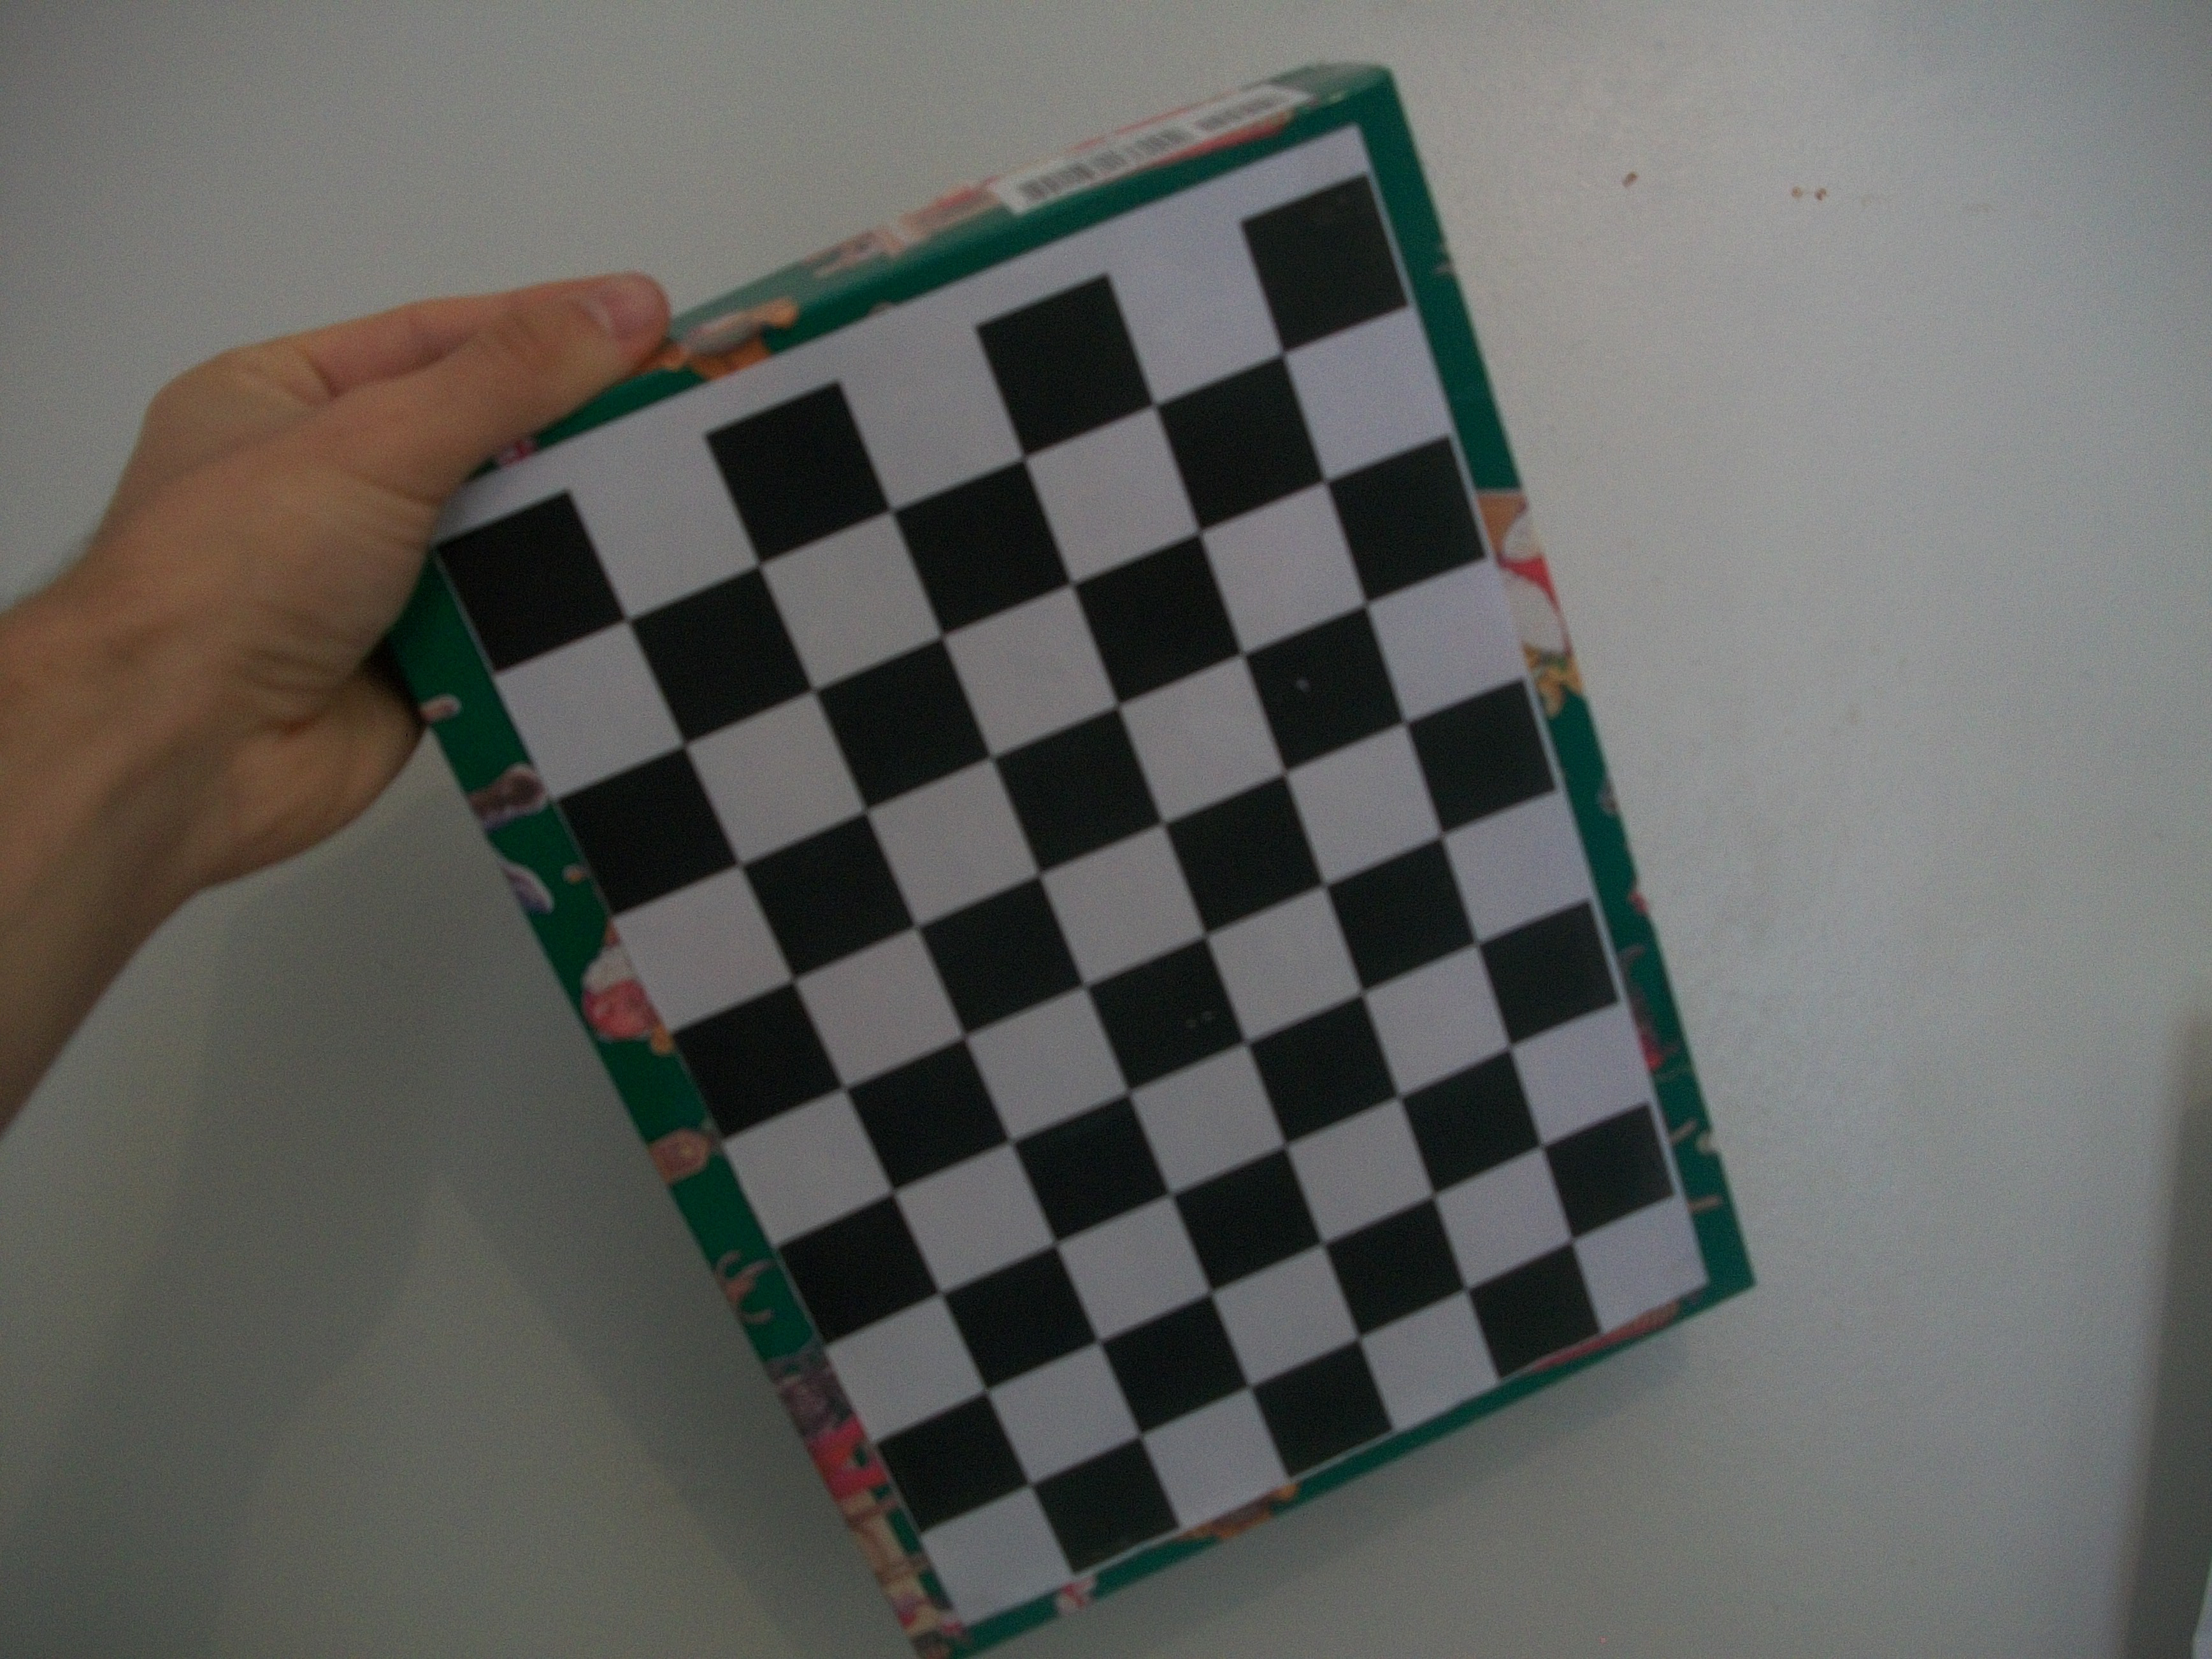
\includegraphics[width=2.8in]{images/im1}
  		\captionof{figure}{$f $ = characters\_test\_pattern.}
		\end{minipage}
		

		\begin{minipage}{\linewidth}
  		\centering
  		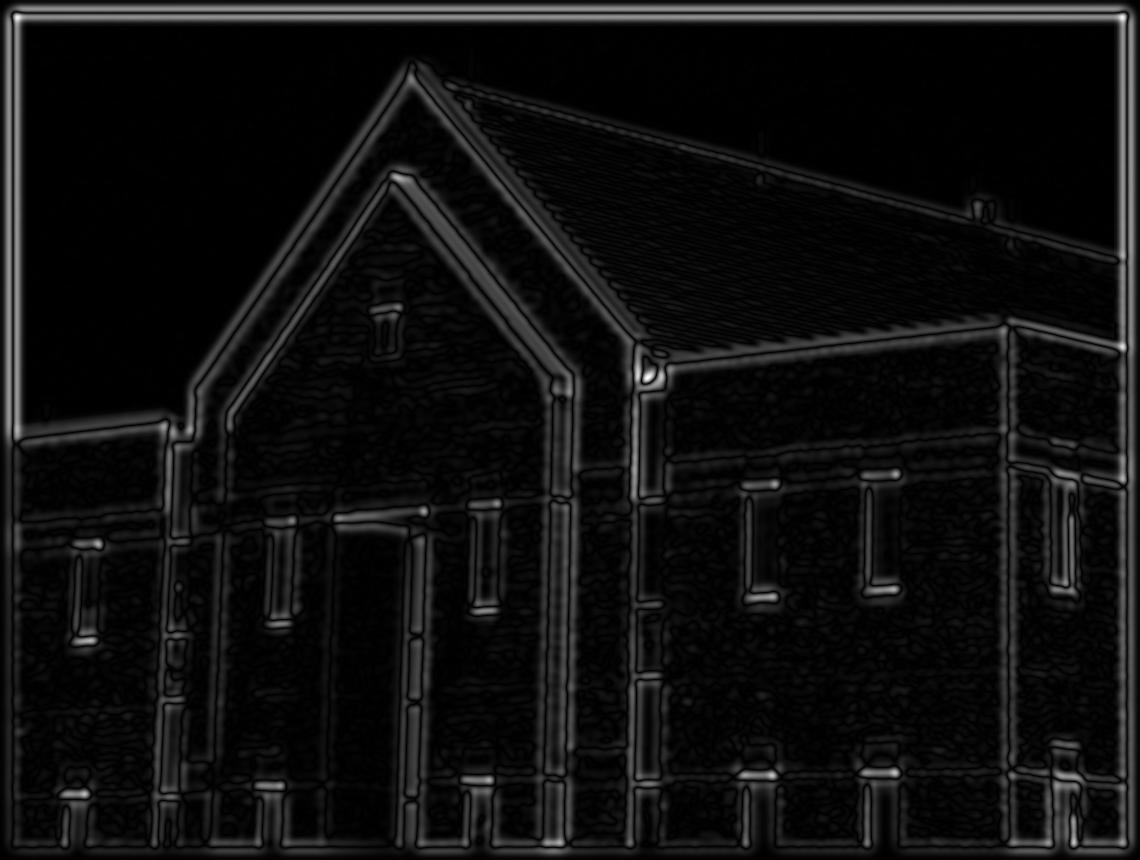
\includegraphics[width=2.8in]{images/im2}
  		\captionof{figure}{$fpa$ = $f $ com preenchimento.}
		\end{minipage}
 		

		\begin{minipage}{\linewidth}
  		\centering
  		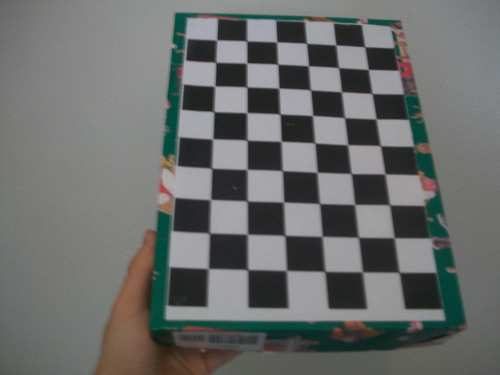
\includegraphics[width=2.8in]{images/im3}
  		\captionof{figure}{$Fpa$ = $DFT$ da $fpa$. Para tornar$-$la vis\'ivel extrapolou$-$se para que qualquer pixel diferente de preto fosse branco. }
		\end{minipage}
 		
 
		\begin{minipage}{\linewidth}
  		\centering
  		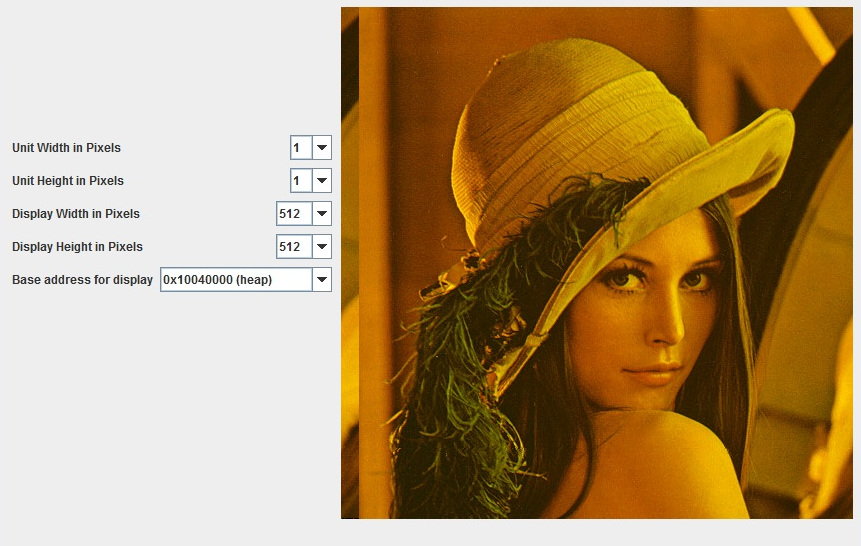
\includegraphics[width=2.8in]{images/im4}
  		\captionof{figure}{$Fpad$ = $Fpa$ deslocada no novo dom\'inio. Usou$-$se o mesmo m\'etodo da  $Fpa $ para torn\'a$-$la vis\'ivel.}
		\end{minipage}		
 		
\centering
\textbf{IDEAL PASSA BAIXAS}

		\begin{minipage}{\linewidth}
  		\centering
  		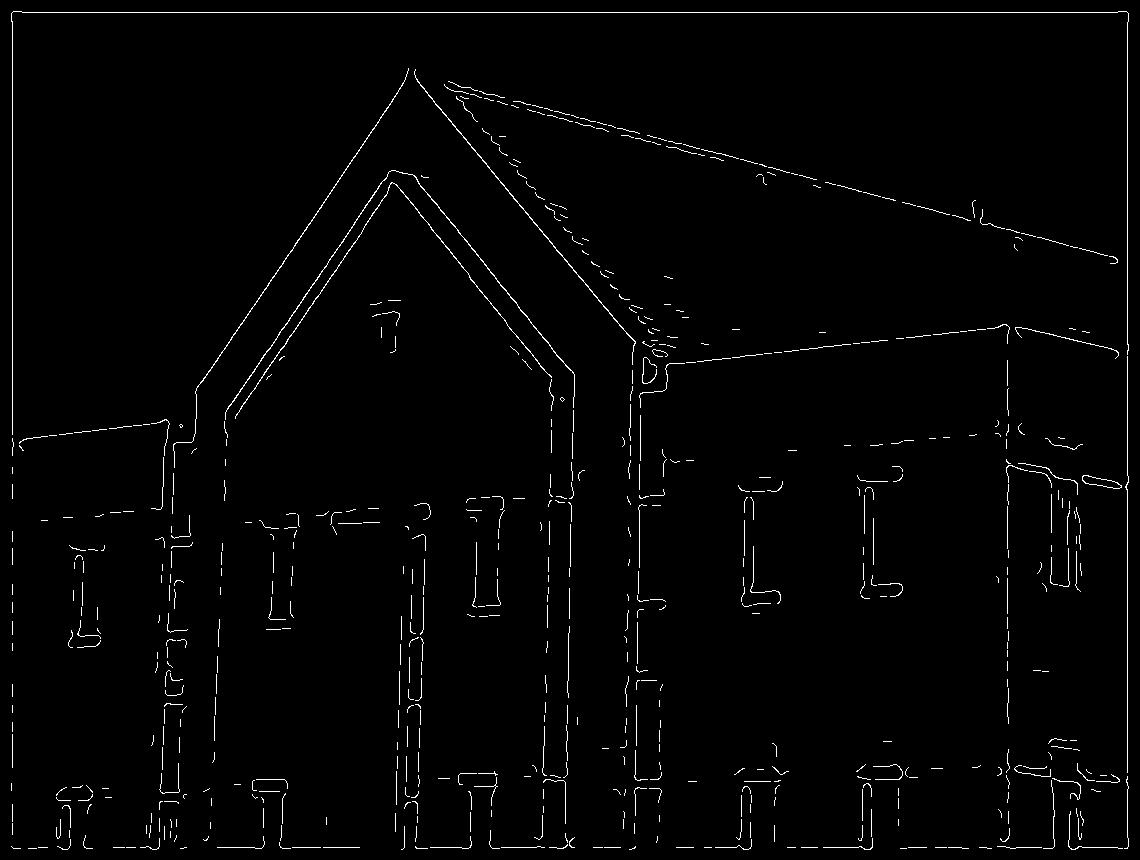
\includegraphics[width=2.8in]{images/im5}
  		\captionof{figure}{$Gpad\_1$ = resultado da multiplica\c{c}\~ao do filtro ideal passa baixas pela $Fpad$.}
		\end{minipage}
		 		

	
\section{Conclus\~ao} 
\label{sec:meth} 

Atrav\'es do uso de ferramentas matem\'aticas ajustadas para representa\c{c}\~oes discretas pode$-$se construir imagens de aproxima\c{c}\~oes ou passa$-$baixas, que \'e caracterizada por borrar e imagens de detalhes ou passa$-$altas, caracterizada pelo agu\c{c}amento e melhora do contraste.

\section{Refer\^encias} 
\label{sec:meth} 

[1] R. C. Gonzalez and R. E. Woods, Digital Image Processing,
Prentice-Hall, EUA, 2nd edition, 2002.
\end{document}